%allocazione tempo 
%
%2 minuti "a cosa servono"
%2 minuti "qubit e porte+ full adder e sqrt not"
%2 minuti "interferenza e entanglement + errori quantistici + confronto computazione analogica"
%2 minuti "error correction e teorema della soglia"
%




%uno speedup polinomiale non rompe la barriera della trattabilità 
%o intrattabilità dei problemi 


\documentclass[aspectratio=169]{beamer}
\usepackage[utf8]{inputenc}
\usepackage{graphicx}
\usepackage{amssymb}
\usepackage{amsfonts}
\usepackage{amsmath}
\usepackage{braket}
\usepackage{tikz}
\usepackage{float}
\usepackage{hyperref}
\usepackage{subcaption}
\usetikzlibrary{quantikz2}
\usepackage{pgfplots}
\usetheme{Copenhagen}
\usecolortheme{beaver}

\title{Quantum errors and error correction tecniques}

\author{Alessio Delli Colli}

\date{September 2024}

\begin{document}

\maketitle

%i numeri sono tutti figli legittimi della matematica
%l'algoritmo di Shor o sue opportune varianti potrebbero risolvere 
%il problema della Fattorizzazione e il problema del lograritmo discreto anche su 
%curve ellittiche. 
%potrebbero e non possono perchè l'hardware disponibile al momento non è ancora adatto 
%a questo tipo di computazione. 
%il numero più alto che si è riusciti a fattorizzare con l'algoritmo di Shor è 21,
%anche il 35 è stato tentato ma senza successo perche la propagazione degli 
%errori ha reso il risultato inutilizzabile
%

\begin{frame}
	\frametitle{Scopo del calcolo quantistico}
	\textbf{Permette di affrontare problemi computazionali "difficili"}

	\pause
	\vspace{30pt}
	\begin{itemize}
		\item problemi di ricerca con l'algoritmo di Grover
		      \vspace{30pt}
		      \pause
		\item fattorizzazione e calcolo del logaritmo discreto con l'algoritmo di Shor.


	\end{itemize}
	\vspace{20pt}
	\pause
	Ma presenta delle criticità...
	\pause
	gli errori.
\end{frame}


%parla del nome circuito
%descrizione del 
\begin{frame}
	\frametitle{Qubits}
	\begin{itemize}
		\item semplici sistemi quantistici
		      \pause
		\item modellati da uno spazio di Hilbert 2-dimensionale
		      \pause
		\item il loro stato può essere rappresentato in vari modi:

	\end{itemize}

	\vspace{10pt}

	\noindent
	\begin{minipage}{0.5\textwidth}
		\begin{center}
			\textbf{Vettore di stato}
		\end{center}
		\begin{equation*}
			\alpha \ket{0} + \beta \ket{1}
		\end{equation*}
		\vspace{10pt}

		le due rappresentazioni sono legate dalla seguente relazione:

		\begin{equation*}
			\ket{\psi} = \cos{\dfrac{\theta}{2}}\ket{0}+e^{i\phi}\sin{\dfrac{\theta}{2}}\ket{1} \\
		\end{equation*}
	\end{minipage}
	\hfill
	\begin{minipage}{0.48\textwidth}
		\begin{center}
			\textbf{Sfera di Bloch}
		\end{center}
		\begin{figure}
			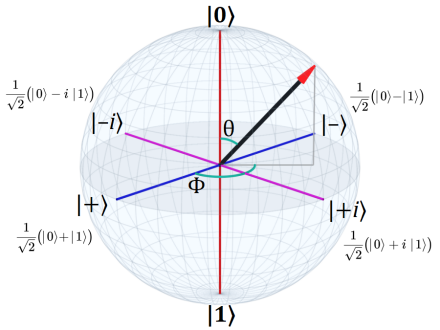
\includegraphics[scale=0.3]{bloch-sphere.png}
		\end{figure}
	\end{minipage}
\end{frame}

\begin{frame}
	\frametitle{Porte quantistiche}

	\begin{itemize}
		\item i qubit sono fatti interagire grazie a delle porte.
		      \pause
		\item queste modificano lo stato applicando ad esso un operatore unitario.
		      \pause
		\item possono essere viste come rotazioni della sfera di Bloch.
		      \pause
		\item vengono composte a formare reti
		      \pause
		\item le porte più comuni sono:
	\end{itemize}

	\vspace{10pt}

	\begin{minipage}{0.24\textwidth}
		\begin{center}
			\textbf{Porte di Pauli}\\
			\vspace{10pt}
			\begin{quantikz}
				\gate{X}
			\end{quantikz}
			\begin{quantikz}
				\gate{Y}
			\end{quantikz}
			\begin{quantikz}
				\gate{Z}
			\end{quantikz}
		\end{center}

	\end{minipage}
	\begin{minipage}{0.24\textwidth}
		\begin{center}
			\textbf{Porte di Fase}\\
			\vspace{10pt}
			\begin{quantikz}
				\gate{S}
			\end{quantikz}
			\begin{quantikz}
				\gate{T}
			\end{quantikz}
			\begin{quantikz}
				\gate{P}
			\end{quantikz}
		\end{center}

	\end{minipage}
	\begin{minipage}{0.24\textwidth}
		\begin{center}
			\textbf{Porta di Hadamard}\\
			\vspace{10pt}
			\begin{quantikz}
				\gate{H}
			\end{quantikz}
		\end{center}
	\end{minipage}
	\begin{minipage}{0.24\textwidth}
		\begin{center}
			\textbf{Not controllato}\\
			\vspace{10pt}
			\begin{quantikz}
				\qw & \ctrl{1} & \qw \\
				\qw & \targ{} & \qw
			\end{quantikz}
		\end{center}
	\end{minipage}

\end{frame}

%attenzione questo non vuol dire che un computer quantistico possa calcolare una funzione
%non calcolabile da una macchina di Turing ma solamente che si ha una maggiore flessibilità 
%a livello circuitale
%
\begin{frame}{Esempi di reti}
	\begin{minipage}{0.6\textwidth}
		\centering
		\textbf{Full adder quantistico}
		\scalebox{1.5}{
			\begin{quantikz}
				\lstick{$\ket{a}$}     & \ctrl{2}  & \ctrl{1}  & \qw      & \qw      & \ctrl{1}  & \rstick{$\ket{a}$} \qw \\
				\lstick{$\ket{b}$}     & \ctrl{2}  & \targ{}   & \ctrl{1} & \ctrl{1} & \targ{}   & \rstick{$\ket{b}$} \qw \\
				\lstick{$\ket{c_{in}}$} & \qw      & \qw      & \ctrl{1} & \targ{}  & \qw       & \rstick{$\ket{s}$} \qw \\
				\lstick{$\ket{0}$}     & \targ{}   & \qw      & \targ{}  & \qw      & \qw       & \rstick{$\ket{c_{out}}$} \qw \\
			\end{quantikz}
		}
	\end{minipage}
	\pause
	\vspace{-20pt}
	\begin{flushright}
		\begin{minipage}{0.6\textwidth}
			\centering
			\textbf{Radice quadrata del not}\\
			\scalebox{2}{
				\begin{quantikz}
					\qw & \gate{H} & \gate{S} & \gate{H} & \qw
				\end{quantikz}
			}
		\end{minipage}
	\end{flushright}
\end{frame}
\begin{frame}{Esempi di reti}
	\begin{minipage}{0.48\textwidth}
		\centering
		\textbf{Interferometro di Ramsey}
		\scalebox{2}{
			\begin{quantikz}
				\qw & \gate{H} & \gate{P}	& \gate{H} & \qw
			\end{quantikz}
		}
	\end{minipage}
	\pause
	\begin{flushright}
		\begin{minipage}{0.5\textwidth}
			\centering
			\textbf{Generatore degli stati di Bell}
			\scalebox{2}{
				\begin{quantikz}
					\qw & \gate{H} & \ctrl{1}	& \qw \\
					\qw &    \qw   & \targ{} &  \qw
				\end{quantikz}
			}
		\end{minipage}
	\end{flushright}


\end{frame}
%nonostante il sistema sia inesorabilmente legato con il mondo esterno noi vogliamo 
%perdere questo legame all'interno della nostra rappresentazione. 
%perche il ondo esterno non lo possiamo misurare, non lo possiamo influenzare in 
%maniera apprezzabile. 
%il mondo dei qubits continuo assomiglia molto di piu al mondo discreto dei bits 
%che al mondo continuo dei qubit 

\begin{frame}
	\frametitle{Correzione degli errori su sistemi classici e quantistici}

	\begin{minipage}{0.32\textwidth}
		\centering
		\textbf{Calcolatore digitale}
		\begin{figure}
			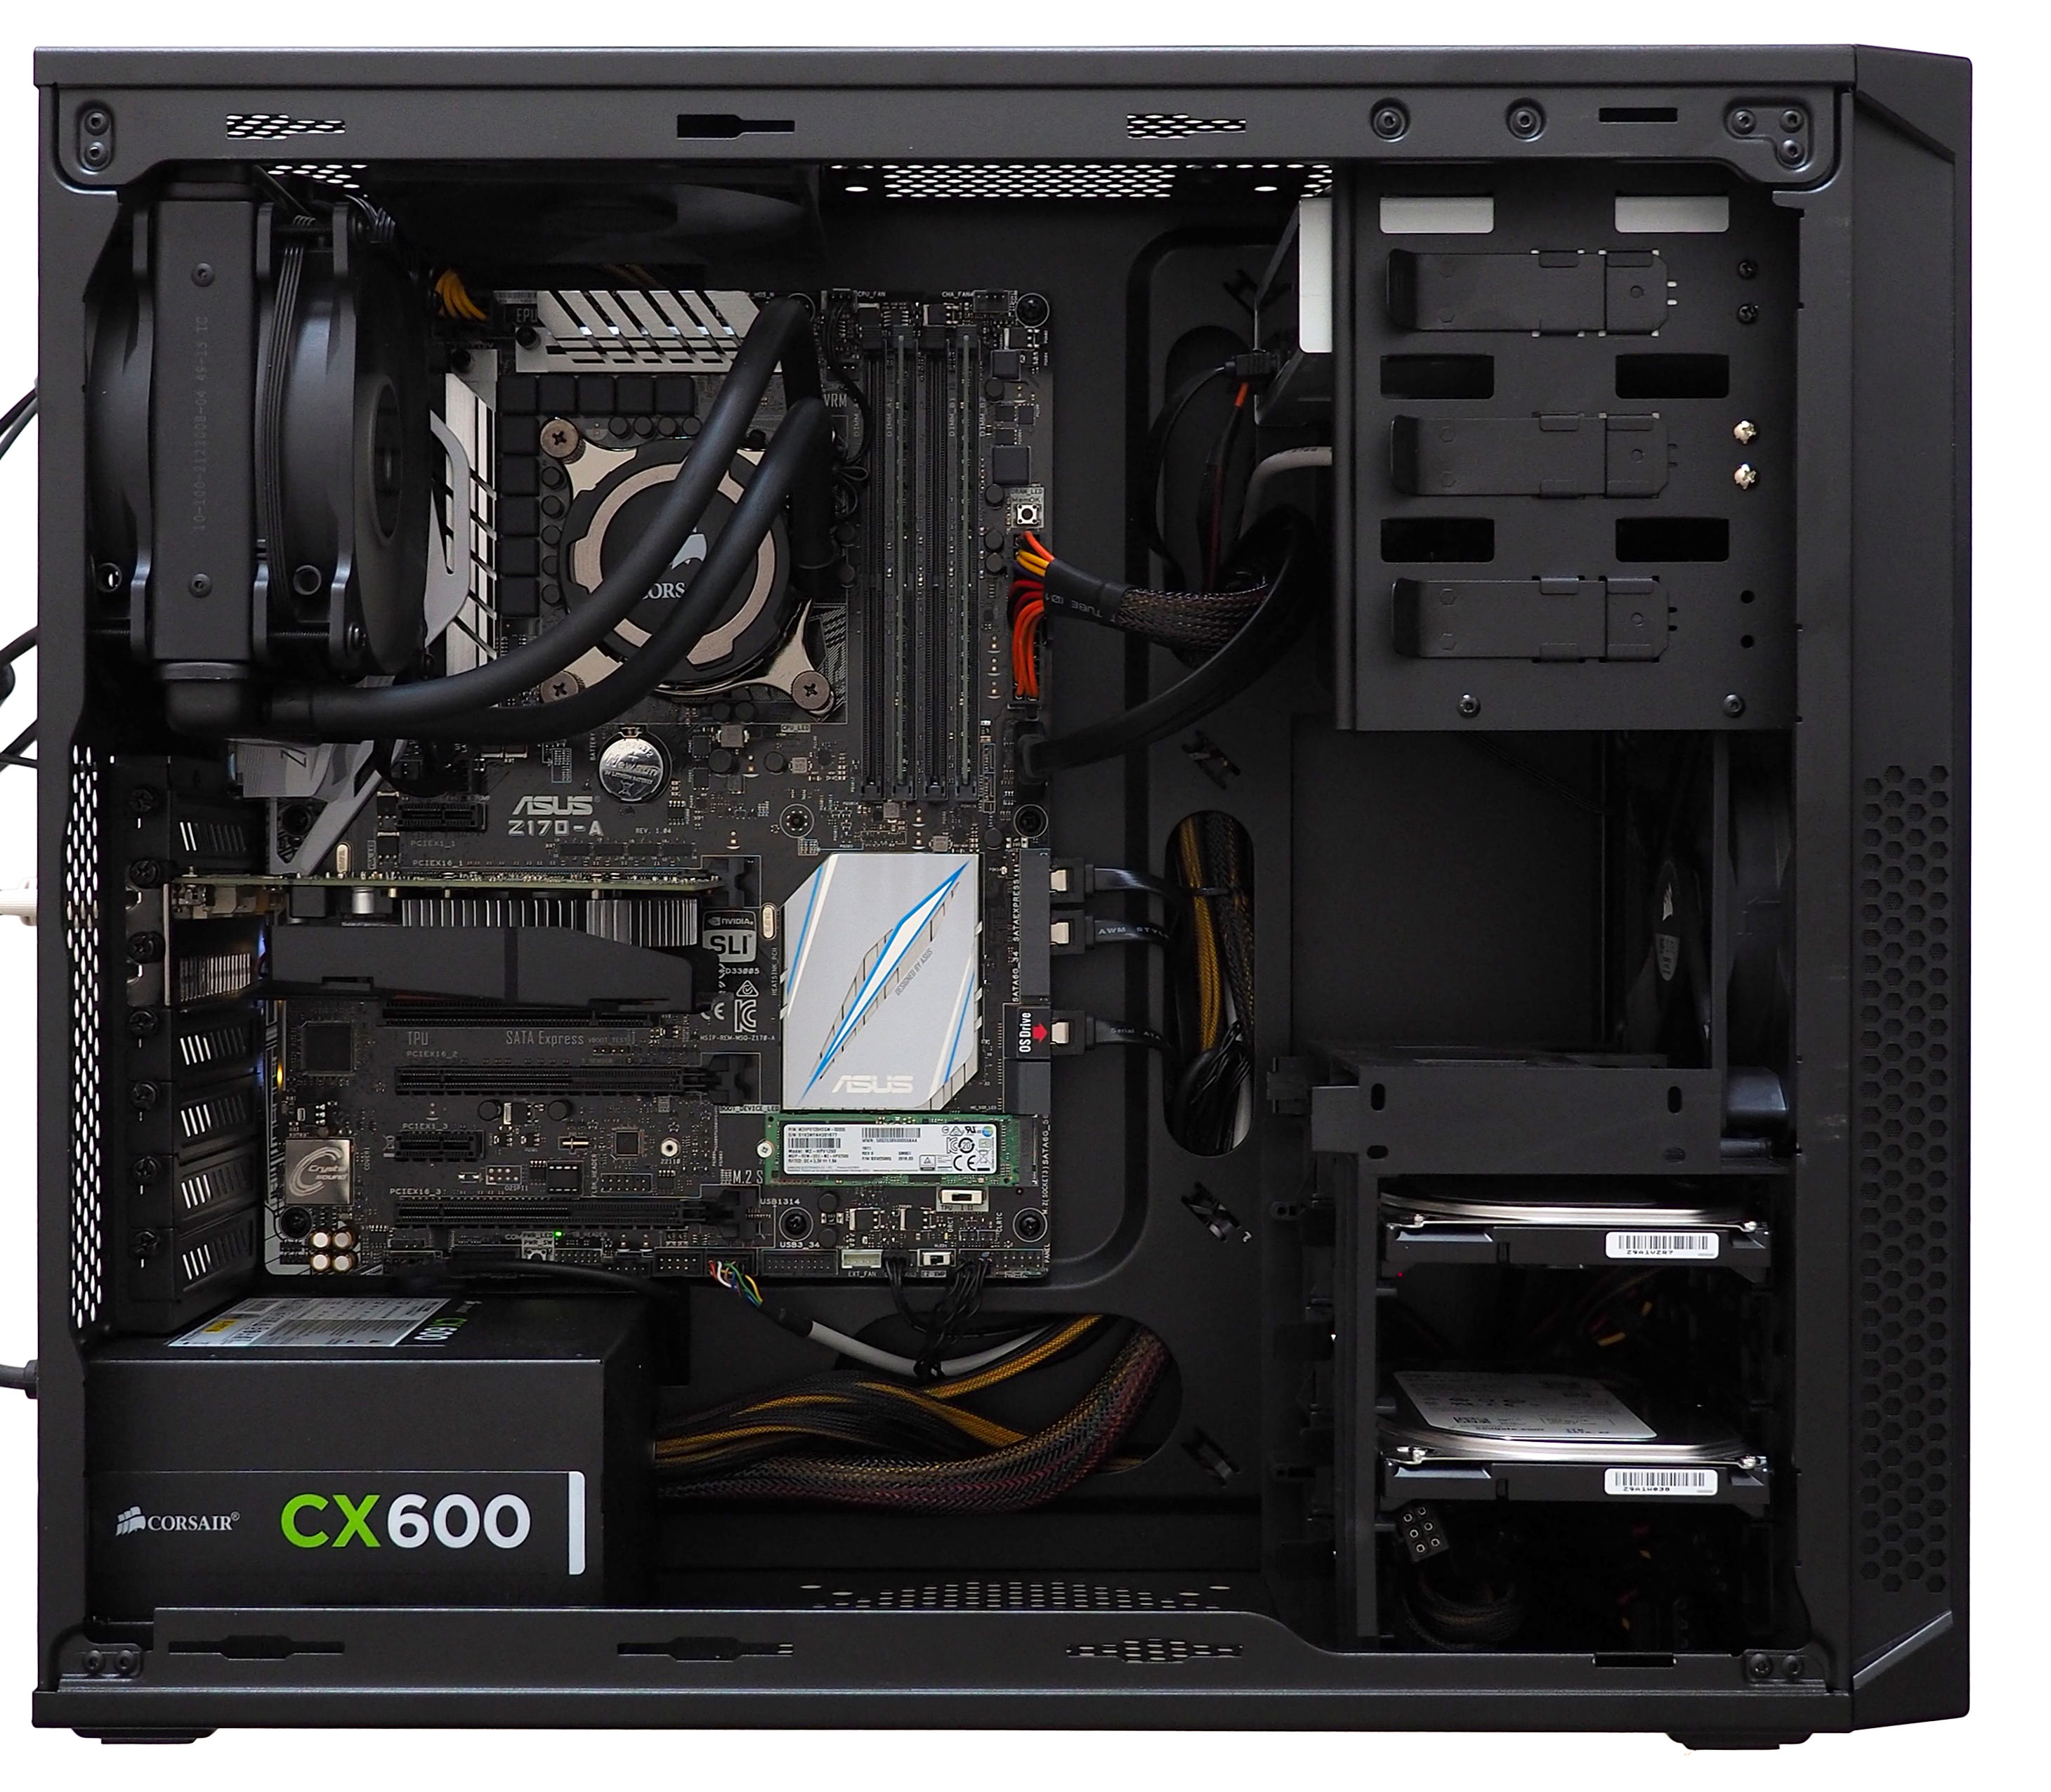
\includegraphics[scale=0.215]{digitale.jpg}
		\end{figure}
		finiti stati, \\
		finite sindromi
	\end{minipage}
	\pause
	\begin{minipage}{0.32\textwidth}
		\centering
		\textbf{Calcolatore analogico}
		\begin{figure}
			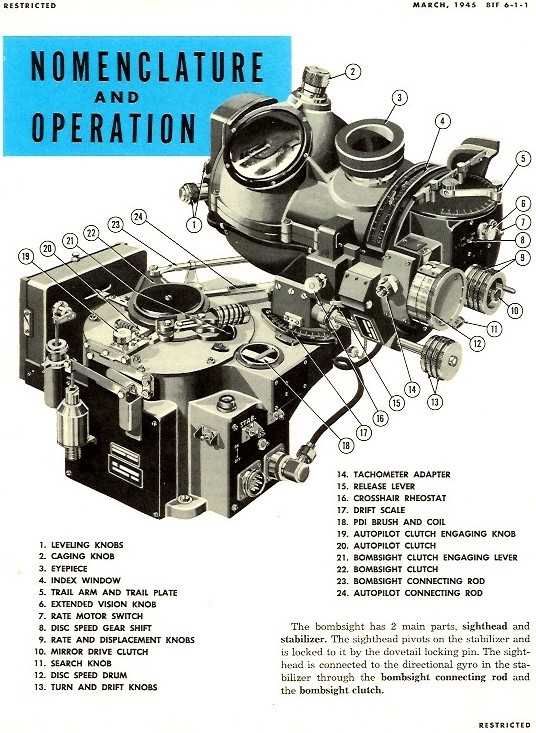
\includegraphics[scale=0.175]{analogico.jpg}
		\end{figure}
		infiniti stati, \\
		infinite sindromi
	\end{minipage}
	\pause
	\begin{minipage}{0.32\textwidth}
		\centering
		\textbf{Calcolatore quantistico}
		\begin{figure}
			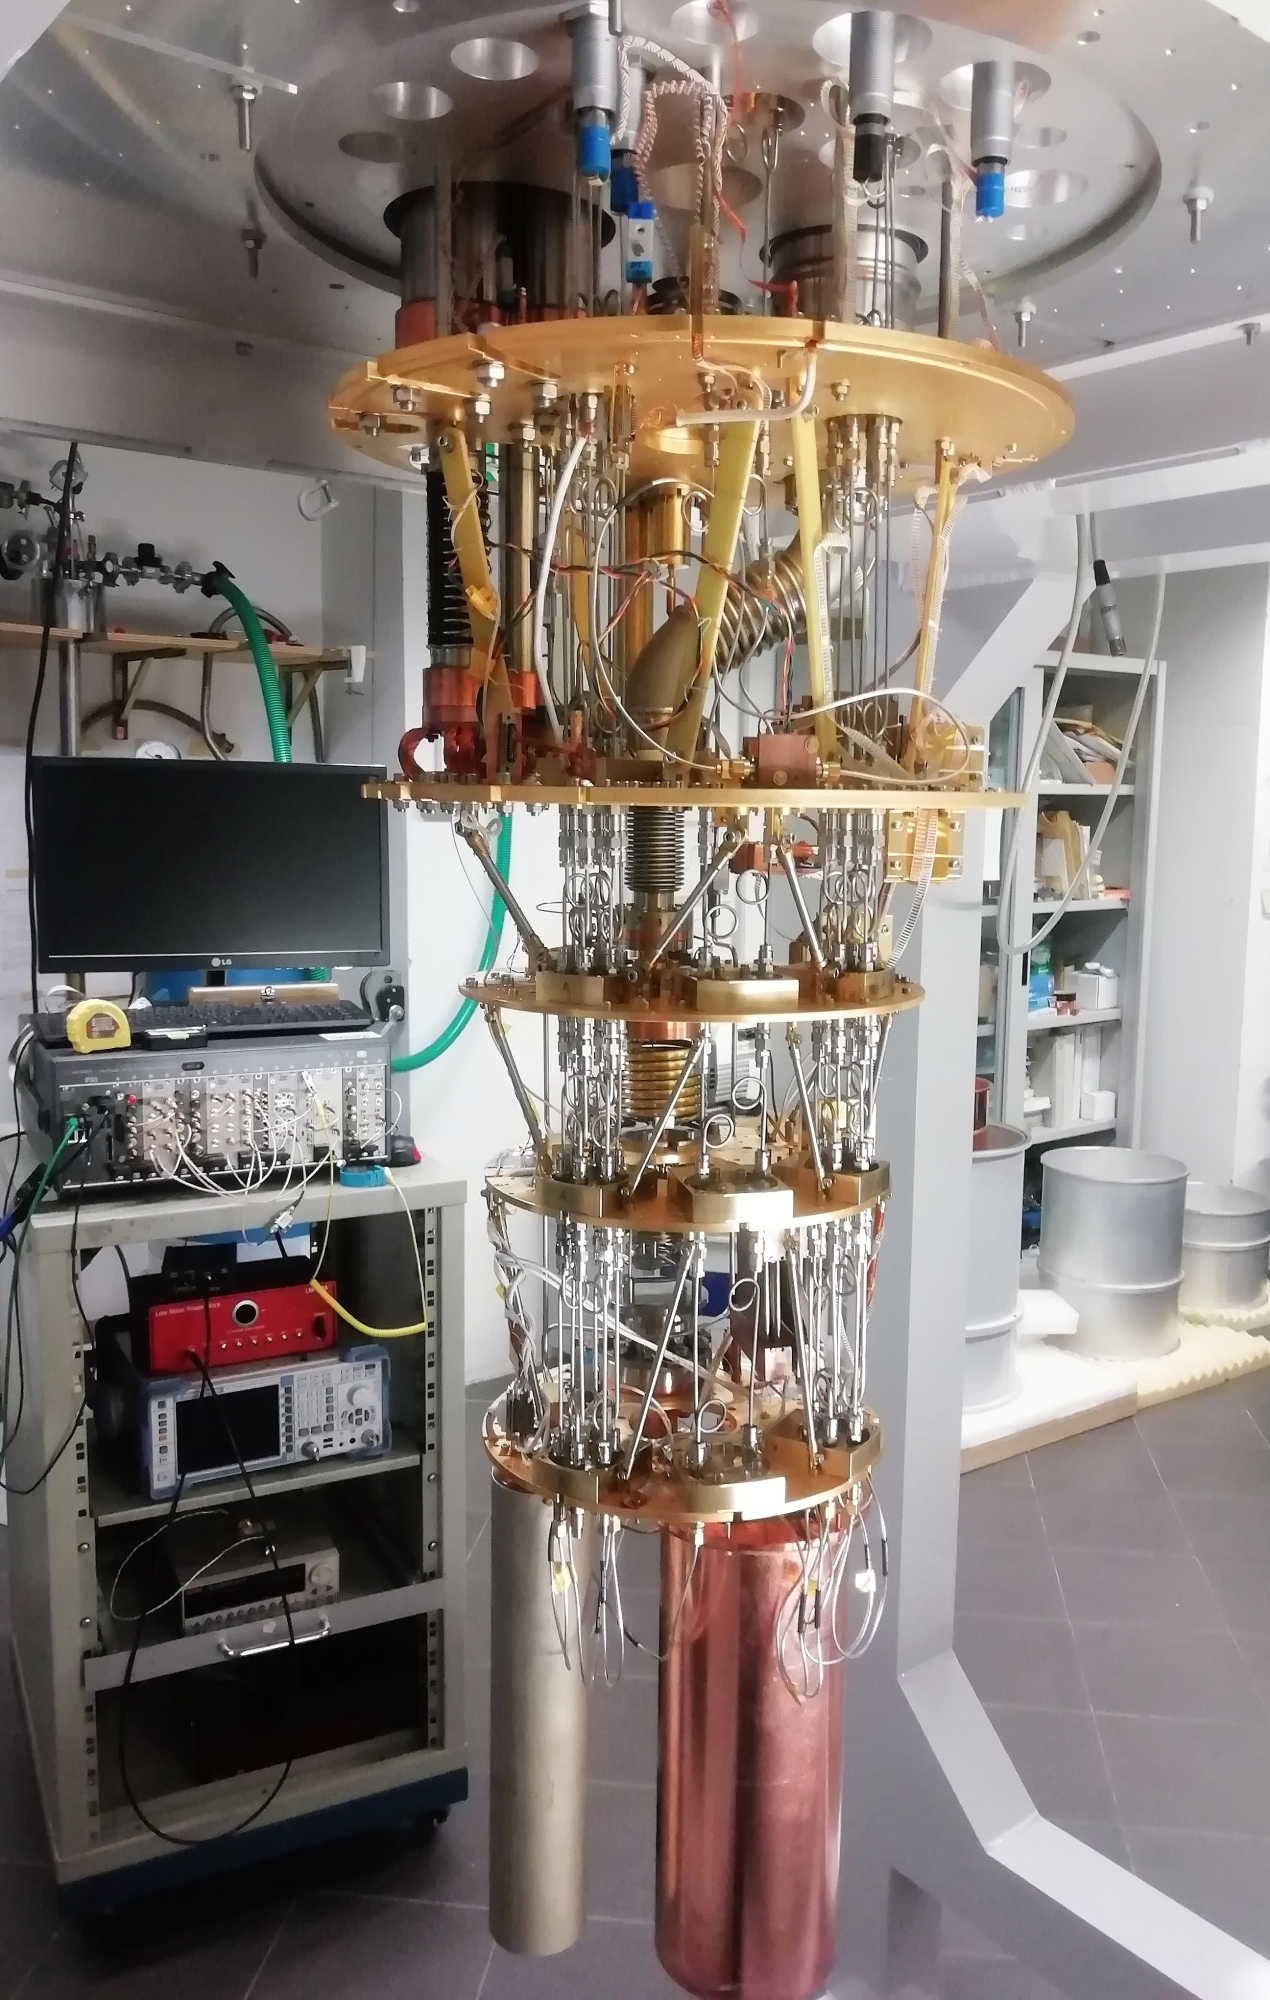
\includegraphics[scale=0.08]{quantistico.jpeg}
		\end{figure}
		infiniti stati, \\
		finite sindromi
	\end{minipage}

\end{frame}

\begin{frame}
	\frametitle{Difficoltà nel caso quantistico}
\end{frame}

\begin{frame}
	\frametitle{Codici di correzione quantistici}
\end{frame}

\begin{frame}
	\begin{center}
		\textbf{\LARGE Grazie per l'attenzione.}
	\end{center}
\end{frame}
\end{document}
